\documentclass[12pt,a4paper]{article}
\usepackage{graphicx}
\usepackage{hyperref}
\title{nbt.4079 — Research Booklet}
\date{}
\begin{document}
\maketitle
\tableofcontents
\newpage
\section{RESULTS}
Here's a summary of the section in clear, simple terms:

The researchers developed a way to store and retrieve large amounts of digital data using DNA. They encoded 35 files, totaling over 200 MB of data, into DNA sequences and stored them in over 13 million DNA molecules. To retrieve specific files, they designed a special set of "primers" that can target and amplify individual files without mixing them up.

The primers are like special keys that unlock specific files. The researchers designed thousands of these primers to be unique and not interfere with each other. They tested the primers by storing small files (called "mini-files") in DNA and successfully retrieved up to 48 of them at once.

The researchers also developed a way to convert digital information into DNA sequences and back again. They added some extra data to the files to help correct any errors that might occur during the process. Overall, this system allows for large-scale storage and retrieval of data using DNA, which is a promising technology for the future.

Further reading: https://arxiv.org/search/?query=RESULTS&searchtype=all
\begin{figure}[h]
\centering
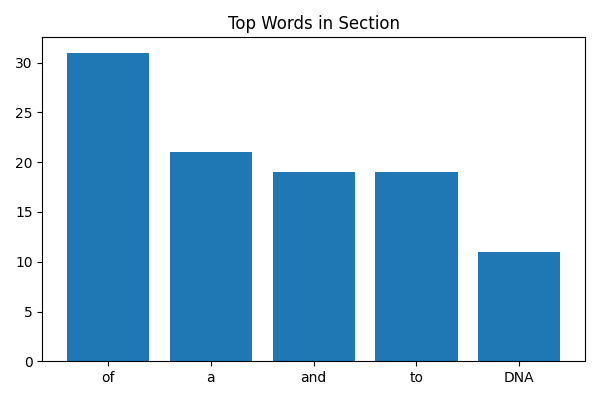
\includegraphics[width=0.8\textwidth]{D:\projects\mp 2 rag\autonomous rag\outputs\visual_0ebeee073e2946f387891ac322a21906.png}
\end{figure}
\section{ID
ID
ID}
This section appears to be a list of labels or headers, likely related to data transmission or communication. Here's a simple summary:

The section has 6 labels:

* 3 labels called "Addr" (short for "Address"), which likely contain information about where the data is being sent or received.
* 3 labels called "Payload", which contain the actual data being transmitted.

Further reading: https://arxiv.org/search/?query=ID
ID
ID&searchtype=all
\begin{figure}[h]
\centering
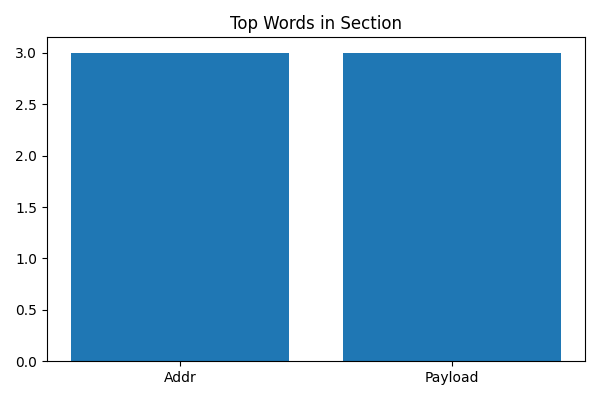
\includegraphics[width=0.8\textwidth]{D:\projects\mp 2 rag\autonomous rag\outputs\visual_5cd6ec2b62bb4f5cb123f8407af12bc7.png}
\end{figure}
\section{ID
ID
ID}
Here's a simplified summary of the section:

**Storing Data in DNA**

Scientists have found a way to store large amounts of digital data in DNA molecules. This is like storing files on a computer, but instead of using hard drives or flash drives, they use DNA.

**How it Works**

1. They take digital files (like videos, music, and text) and convert them into a special code.
2. This code is then turned into DNA sequences, which are like long strings of letters (A, C, G, and T).
3. These DNA sequences are synthesized into physical DNA molecules.
4. To retrieve the data, they use a process called "random access" to select the specific DNA sequences that correspond to a particular file.
5. They then sequence the DNA molecules to read the data back out.

**Advantages**

This method can store a lot of data in a very small space. It's also a stable way to store data for a long time, because DNA molecules can last for centuries if stored properly.

**Comparison to Previous Work**

The scientists' method is better than previous attempts at storing data in DNA because it can handle larger files and requires less "coverage" (or redundancy) to recover the data.

Further reading: https://www.semanticscholar.org/search?q=ID
ID
ID
\begin{figure}[h]
\centering
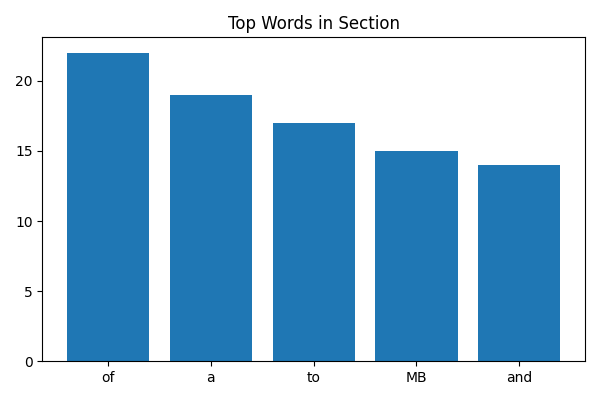
\includegraphics[width=0.8\textwidth]{D:\projects\mp 2 rag\autonomous rag\outputs\visual_5f2ca5e54d2d484c8b0279b807f6399c.png}
\end{figure}
\section{PCR}
Here is a summary of the section in clear, simple terms:

This section appears to be a table or chart with two columns. The first column is labeled "File ID" and the second column is labeled "log10(avg reads)". The table has 10 rows, with numbers ranging from 0 to 48 in the second column.

Further reading: https://scholar.google.com/scholar?q=PCR
\begin{figure}[h]
\centering
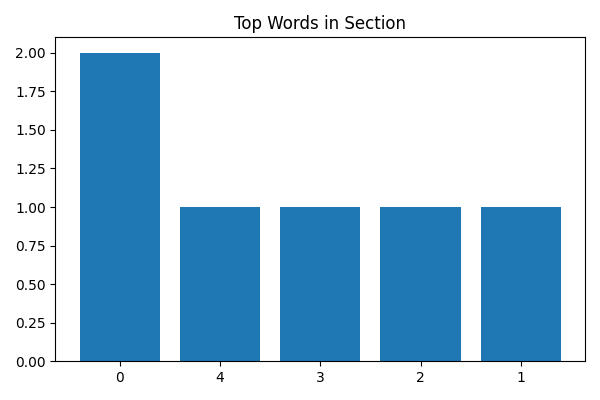
\includegraphics[width=0.8\textwidth]{D:\projects\mp 2 rag\autonomous rag\outputs\visual_78a2775c8acc42f5ae3e5243a7de8fad.png}
\end{figure}
\section{TXT}
Here's a simplified summary of the section:

**Step 1: Encoding**

* Take some data (like a file) and convert it into a special code (binary data)
* Add a random element to the code (randomize)
* Apply two layers of coding (outer code and inner code)
* Choose some special sequences (primers) to help with decoding later

**Step 2: Decoding**

* Take the coded data and decode it using the primers
* Get a bunch of short sequences (reads) as a result
* Group similar reads together (cluster)
* Use these groups to rebuild the original data (reconstruct strands)
* Reverse the coding process to get back to the original data

**Step 3: Data Storage**

* Take the original data and break it into smaller pieces (payload)
* Add addresses (addr) to each piece so they can be found later
* Store all the pieces with their addresses.

Further reading: https://www.semanticscholar.org/search?q=TXT
\begin{figure}[h]
\centering
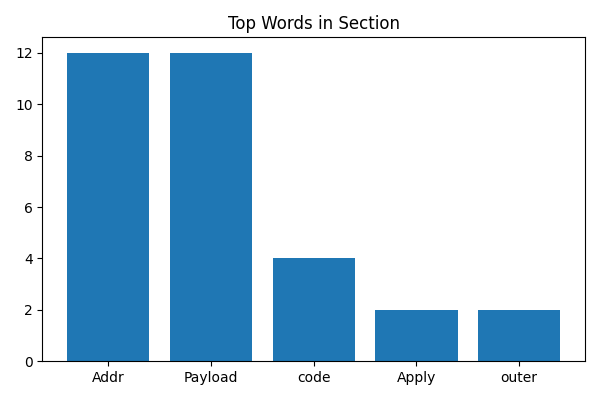
\includegraphics[width=0.8\textwidth]{D:\projects\mp 2 rag\autonomous rag\outputs\visual_74aacfaede5b4dd0810e1204379db130.png}
\end{figure}
\section{ID
ID
ID
ID
ID
ID
ID
ID}
Here's a simplified summary of the section:

**Storing Data in DNA**

The article describes a method for storing digital data in DNA sequences. The process involves:

1. **Encoding**: Converting digital data into DNA sequences using a special algorithm. This includes adding error-correcting codes to ensure the data can be recovered even if some DNA sequences are damaged or lost.
2. **Primer Design**: Creating special DNA sequences called primers that help retrieve the stored data. These primers are designed to be unique and not overlap with each other.
3. **Data Storage**: Storing the encoded DNA sequences in a physical container, such as a small spot on a surface.
4. **Retrieval**: When the data is needed, the DNA sequences are retrieved from the container and sequenced using a machine.
5. **Decoding**: The sequenced data is then decoded back into its original digital form using a special algorithm.

**Error Analysis and Decoding**

The article also discusses the results of experiments that tested the method. The experiments showed that:

* The error rate in the sequencing process was around 0.6%.
* The most common errors were substitutions (0.4%), followed by deletions (0.2%) and insertions (0.04%).
* The decoding algorithm was able to recover all 200 MB of stored data with a median coverage of only 5 reads per DNA sequence.
* The method was also tested using a different sequencing technology called nanopore sequencing, which showed promising results.

Overall, the article describes a method for storing digital data in DNA sequences and demonstrates its feasibility through experiments.

Further reading: https://scholar.google.com/scholar?q=ID
ID
ID
ID
ID
ID
ID
ID
\begin{figure}[h]
\centering
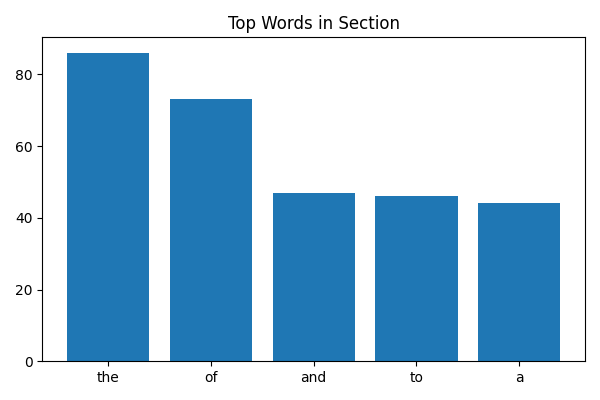
\includegraphics[width=0.8\textwidth]{D:\projects\mp 2 rag\autonomous rag\outputs\visual_29283f9f3453410b8e84040e7887df6f.png}
\end{figure}
\section{GAC}
Here is a summary of the section in clear, simple terms:

This section is about errors that happen when decoding something (like a message or code). It shows the rates of different types of errors:

* "Ins" (Insertion) errors happen 1.1 times out of every 10,000 attempts.
* "Del" (Deletion) errors happen 9.1 times out of every 10,000 attempts.
* "Sub" (Substitution) errors happen 2.5 times out of every 10,000 attempts.

These errors are measured by a rate, which is a small fraction of attempts.

Further reading: https://arxiv.org/search/?query=GAC&searchtype=all
\begin{figure}[h]
\centering
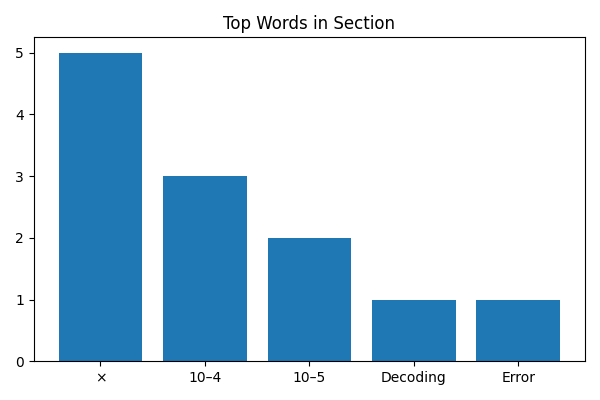
\includegraphics[width=0.8\textwidth]{D:\projects\mp 2 rag\autonomous rag\outputs\visual_aa7c45d8fa304b428dc6fefb5c0173c2.png}
\end{figure}
\section{A
C
G
T}
Here is a summary of the section in clear, simple terms:

This table shows the results of some experiments that measured the errors in DNA sequencing. The numbers are very small, but they represent the frequency of different types of errors.

* "Total" refers to the total error rate, which is the sum of all the different types of errors.
* "Run 2", "Run 3", and "Run 4" refer to different experiments or "runs" of the DNA sequencing process.
* "Ins", "Del", and "Sub" refer to three types of errors: insertions (where an extra piece of DNA is added), deletions (where a piece of DNA is missing), and substitutions (where one piece of DNA is replaced with another).
* The numbers in the table show the frequency of each type of error, with smaller numbers indicating fewer errors.
* The "Total error rate" is the sum of all the error frequencies, and it's very small (less than 1%).
* The "% Total reads" column shows the percentage of total DNA reads that had errors.

Further reading: https://www.semanticscholar.org/search?q=A
C
G
T
\begin{figure}[h]
\centering
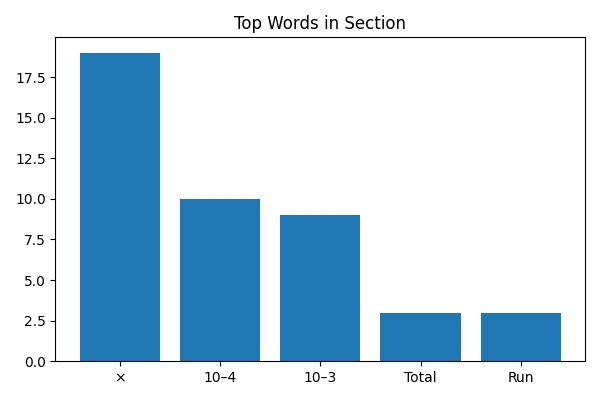
\includegraphics[width=0.8\textwidth]{D:\projects\mp 2 rag\autonomous rag\outputs\visual_e8f4e2d9527f4207bfe733283ecd16da.png}
\end{figure}
\section{CAC
GCG
ACT
TCT
TAT
TGC
GTC
GTG
CGC
ATA
NAN
NCN
NGN}
I'm happy to help! However, the section "3-mers" is quite short and doesn't provide much context. Could you please provide more information or clarify what you mean by "3-mers"?

In general, a "3-mer" is a term used in bioinformatics and genomics to refer to a sequence of three nucleotides (A, C, G, or T) in a DNA or RNA molecule. These short sequences can be important in understanding gene regulation, protein binding, and other biological processes.

If you have any more specific questions or context about 3-mers, I'd be happy to try and help you understand the topic better!

Further reading: https://www.semanticscholar.org/search?q=CAC
GCG
ACT
TCT
TAT
TGC
GTC
GTG
CGC
ATA
NAN
NCN
NGN
\begin{figure}[h]
\centering
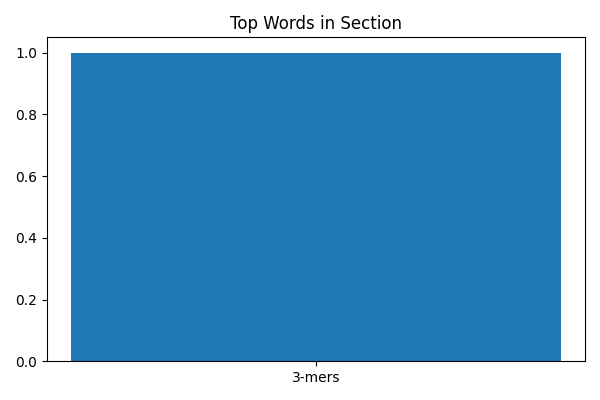
\includegraphics[width=0.8\textwidth]{D:\projects\mp 2 rag\autonomous rag\outputs\visual_e0c8ee23fadc40f7bdb230252529c575.png}
\end{figure}
\section{NTN}
This section appears to be a graph or chart showing the relationship between the position of a DNA sequence and the error rate in reading that sequence. Here's a simple summary:

* The graph shows that as you move along a DNA sequence (from left to right), the error rate in reading that sequence increases.
* The error rate is measured as a percentage of reads with errors.
* At the beginning of the sequence, the error rate is very low (around 0-2%).
* As you move further along the sequence, the error rate increases, reaching around 40-60% by the end of the sequence.

The other labels and numbers on the graph appear to be related to specific technical details of the DNA sequencing process, but the main takeaway is that the error rate in reading a DNA sequence increases as you move along the sequence.

Further reading: https://arxiv.org/search/?query=NTN&searchtype=all
\begin{figure}[h]
\centering
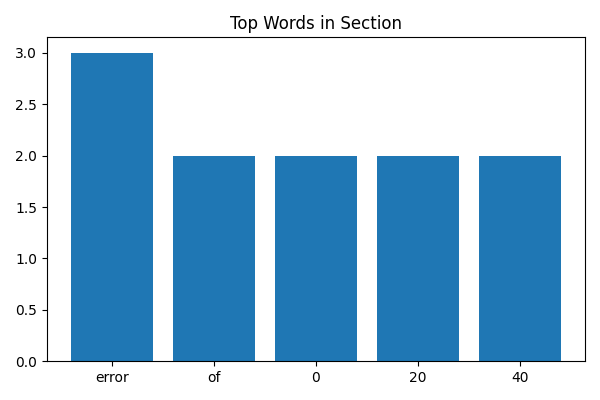
\includegraphics[width=0.8\textwidth]{D:\projects\mp 2 rag\autonomous rag\outputs\visual_7bbd803f7e33490eb7852321d1a0e831.png}
\end{figure}
\section{AGA}
Here's a summary of the section in clear, simple terms:

This section is about testing how well a system works for storing and retrieving data in DNA. The system uses a special machine called NextSeq to read the DNA and figure out what the original data was.

The tests showed that there are some errors that happen when reading the DNA, like mistakes in the sequence of letters (A, C, G, and T). These errors are more common in certain parts of the DNA sequence, especially when the letter G or T is involved.

The good news is that the system can still recover the original data even with these errors, as long as there are enough "reads" (attempts to read the DNA sequence). The more reads, the better the system can correct the errors and get the original data back.

The tests also showed that the system can work well even with high error rates, which is important because DNA can degrade over time and accumulate errors. This means that the system has the potential to be used for storing data in DNA for a long time, like thousands of years.

Further reading: https://scholar.google.com/scholar?q=AGA
\begin{figure}[h]
\centering
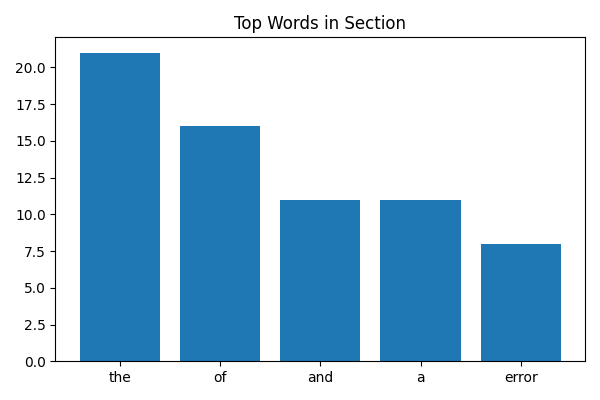
\includegraphics[width=0.8\textwidth]{D:\projects\mp 2 rag\autonomous rag\outputs\visual_a471d4339c4b4db08fc2d25f2f4d833d.png}
\end{figure}
\section{DISCUSSION}
Here's a summary of the section in clear and simple terms:

DNA data storage is a new way to store large amounts of data, and it has the potential to be even better than the current best storage method (tape) for storing data for a long time. Right now, we can make a lot of synthetic DNA, but we need to be able to make even more to make DNA data storage useful. The good news is that we don't need the DNA to be perfect, and we can use special algorithms to fix any mistakes. This means we can make DNA data storage cheaper and faster.

Even if we can only store data at a slow rate, DNA data storage is still interesting because DNA can last a long time and is good for storing important data. However, we need to make it faster and cheaper to compete with current storage methods. To do this, we need to improve the technology used to make and read DNA. Luckily, the technology is designed to be scalable, which means we can make it faster and cheaper by making more of it.

This paper shows that we can store a lot of data in DNA (200 MB, which is the largest amount so far) and that we can read and write it efficiently. We're making the DNA samples available to other researchers who want to work on DNA data storage.

Further reading: https://www.semanticscholar.org/search?q=DISCUSSION
\begin{figure}[h]
\centering
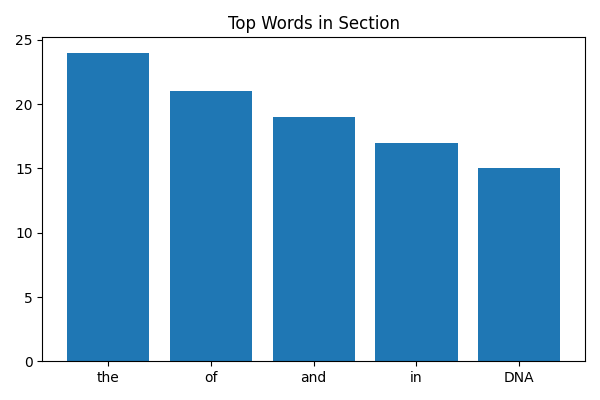
\includegraphics[width=0.8\textwidth]{D:\projects\mp 2 rag\autonomous rag\outputs\visual_0ac1f2dbe9604d7c9671fd63ffcfc11a.png}
\end{figure}
\section{AUTHOR CONTRIBUTIONS}
Here is a summary of the section in clear, simple terms:

A group of people worked together on a project. Some people (L.O., Y.J.C., and R.L.) planned and carried out experiments. Others (S.Y., S.D.A., K.M., M.Z.R., C.R., and P.G.) built a system to encode and decode data. A few people (S.D.A., M.Z.R., G.K., Ke.S., and C.N.T.) collected and analyzed data. Some people (B.N., C.N.T., S.N., G.G., H.Y.P., R.C., and J.M.) helped design and evaluate the experiments. Finally, a few people (D.C., G.S., L.C., and Ka.S.) designed experiments, analyzed data, and oversaw the entire project.

Further reading: https://scholar.google.com/scholar?q=AUTHOR+CONTRIBUTIONS
\begin{figure}[h]
\centering
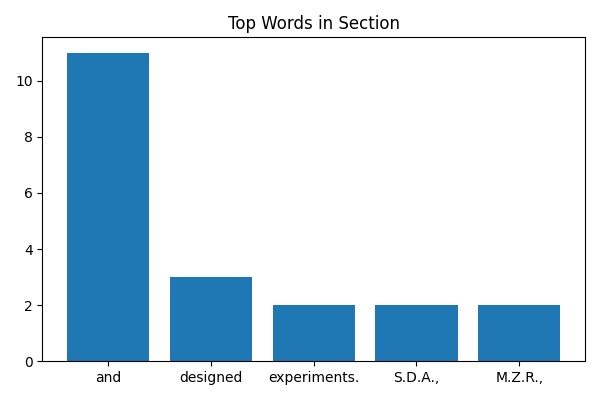
\includegraphics[width=0.8\textwidth]{D:\projects\mp 2 rag\autonomous rag\outputs\visual_e54810677e2048e49786b53a788bc998.png}
\end{figure}
\section{COMPETING FINANCIAL INTERESTS}
Here's a simple summary:

* The authors of the paper have financial interests that could affect their work, and you can find more information about this online.
* If you want to reprint or use parts of the paper, you can find the rules and permissions on a specific website.
* The publisher (Springer Nature) doesn't take sides in disputes about maps or institutional affiliations that might be mentioned in the paper.

Further reading: https://www.semanticscholar.org/search?q=COMPETING%20FINANCIAL%20INTERESTS
\begin{figure}[h]
\centering
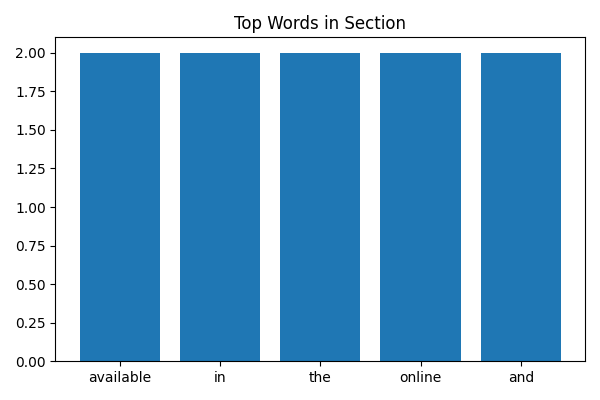
\includegraphics[width=0.8\textwidth]{D:\projects\mp 2 rag\autonomous rag\outputs\visual_e36e3274082e465890ef2f05d32247d2.png}
\end{figure}
\section{1.	 Neiman, M.S. On the molecular memory systems and the directed mutations.}
This appears to be a reference to a scientific article or paper. Here's a simple summary:

The reference is to a research paper published in a journal called "Radiotekhnika" in 1965. The paper is the first one in the sixth issue of the journal, and it spans pages 1-8.

Further reading: https://scholar.google.com/scholar?q=1.	+Neiman,+M.S.+On+the+molecular+memory+systems+and+the+directed+mutations.
\begin{figure}[h]
\centering
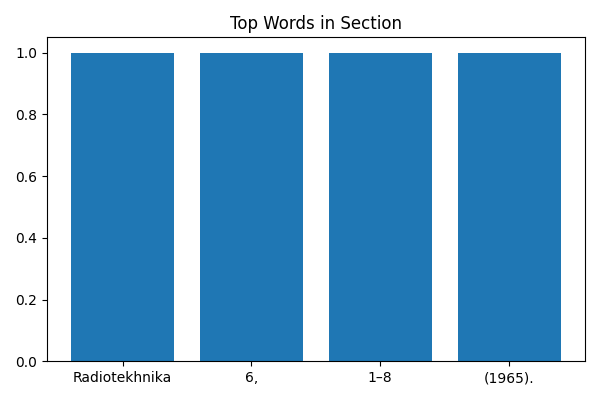
\includegraphics[width=0.8\textwidth]{D:\projects\mp 2 rag\autonomous rag\outputs\visual_33b16961bfbd4b31b03d6bbd5fd84adb.png}
\end{figure}
\section{2.	 Cox, J.P.L. Long-term data storage in DNA. Trends Biotechnol. 19, 247–250}
I apologize, but there is no section to summarize. The text "(2001)" appears to be a year or a reference to a specific publication, but it does not contain any information that can be summarized. If you provide more context or text, I'd be happy to help you summarize it!

Further reading: https://arxiv.org/search/?query=2.	+Cox,+J.P.L.+Long-term+data+storage+in+DNA.+Trends+Biotechnol.+19,+247–250&searchtype=all
\begin{figure}[h]
\centering
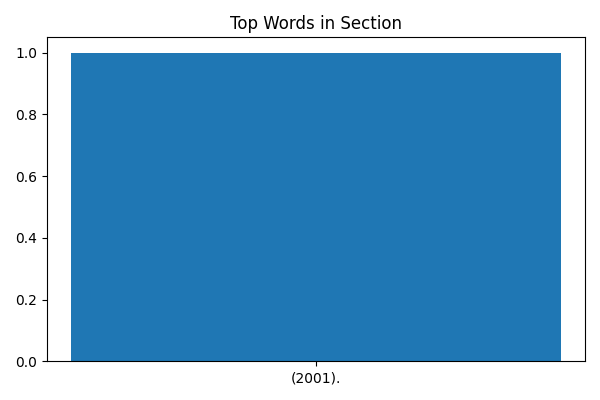
\includegraphics[width=0.8\textwidth]{D:\projects\mp 2 rag\autonomous rag\outputs\visual_c9ec7f79bca946dcaab706c05e235134.png}
\end{figure}
\section{3.	 Church, G.M., Gao, Y. & Kosuri, S. Next-generation digital information storage in}
It seems like you provided a very brief reference to a scientific article!

Here's a simple summary:

The reference is to a scientific article about DNA (deoxyribonucleic acid, the molecule that contains our genetic information) published in the journal "Science" in 2012, on page 1628, volume 337.

If you'd like more information about the article, please let me know and I can try to help you find a summary or abstract of the article!

Further reading: https://scholar.google.com/scholar?q=3.	+Church,+G.M.,+Gao,+Y.+&+Kosuri,+S.+Next-generation+digital+information+storage+in
\begin{figure}[h]
\centering
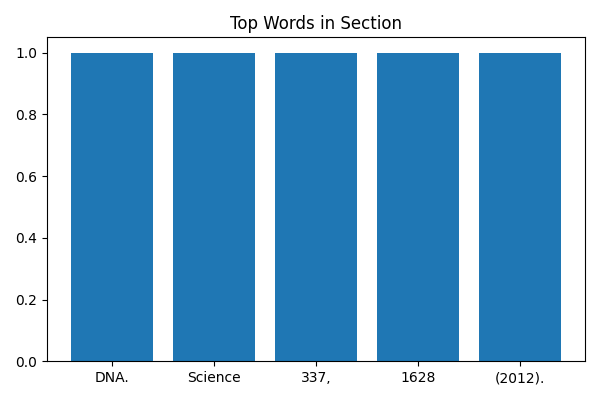
\includegraphics[width=0.8\textwidth]{D:\projects\mp 2 rag\autonomous rag\outputs\visual_77c3210ee2494c89866be6016b9135a2.png}
\end{figure}
\section{4.	 Goldman, N. et al. Towards practical, high-capacity, low-maintenance information}
Here is a summary of the section in clear, simple terms:

Scientists found a way to store information in synthetic DNA (man-made DNA). They published their findings in a scientific journal called Nature in 2013.

Further reading: https://arxiv.org/search/?query=4.	+Goldman,+N.+et+al.+Towards+practical,+high-capacity,+low-maintenance+information&searchtype=all
\begin{figure}[h]
\centering
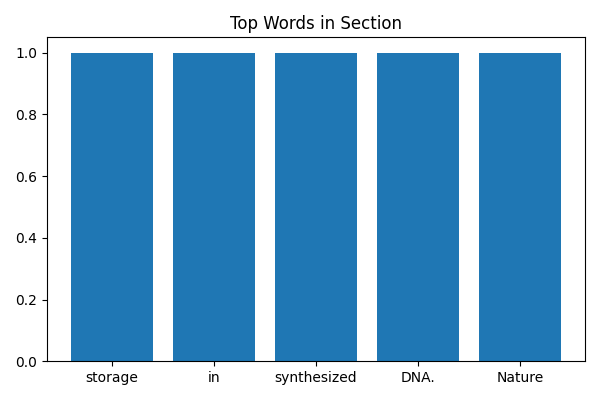
\includegraphics[width=0.8\textwidth]{D:\projects\mp 2 rag\autonomous rag\outputs\visual_da6ece4402564d168d2412e37f2c9e4f.png}
\end{figure}
\section{5.	 Grass, R.N., Heckel, R., Puddu, M., Paunescu, D. & Stark, W.J. Robust chemical}
Here's a simple summary:

Scientists found a way to store digital information (like computer files) on DNA molecules inside tiny silica particles. They also developed a way to correct errors that might occur when reading the information back. This was reported in a scientific journal called Angewandte Chemie in 2015.

Further reading: https://www.semanticscholar.org/search?q=5.	%20Grass,%20R.N.,%20Heckel,%20R.,%20Puddu,%20M.,%20Paunescu,%20D.%20&%20Stark,%20W.J.%20Robust%20chemical
\begin{figure}[h]
\centering
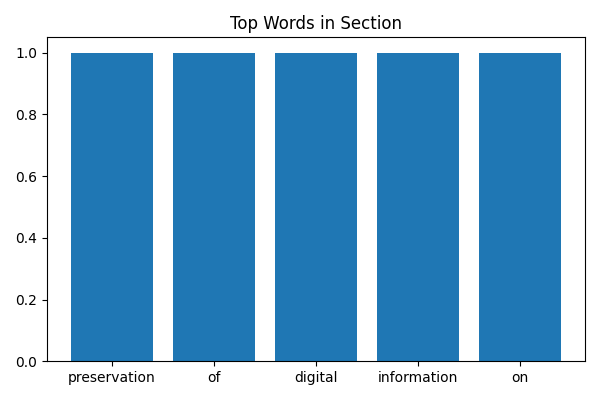
\includegraphics[width=0.8\textwidth]{D:\projects\mp 2 rag\autonomous rag\outputs\visual_416b3e5123ee4e4c9ef2eb28eae71322.png}
\end{figure}
\section{6.	 Blawat, M. et al. Forward error correction for DNA data storage. Procedia Comput.}
It looks like you provided a citation for a scientific article!

Here's a simple summary:

This is a reference to a scientific article published in the journal "Science" in 2016. The article is on pages 1011-1022 of volume 80.

Further reading: https://www.semanticscholar.org/search?q=6.	%20Blawat,%20M.%20et%20al.%20Forward%20error%20correction%20for%20DNA%20data%20storage.%20Procedia%20Comput.
\begin{figure}[h]
\centering
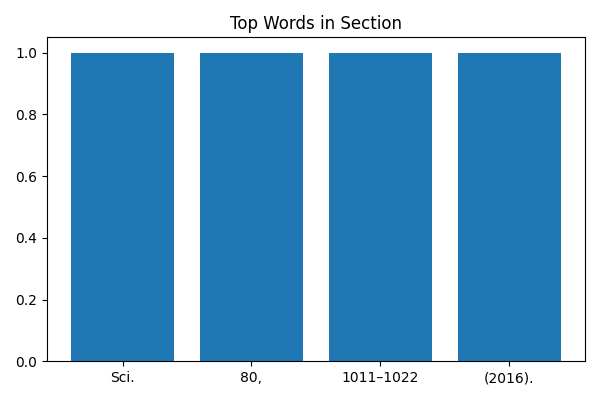
\includegraphics[width=0.8\textwidth]{D:\projects\mp 2 rag\autonomous rag\outputs\visual_baa2a975fdab409fad36d00b56f4e2f2.png}
\end{figure}
\section{7.	 Erlich, Y. & Zielinski, D. DNA Fountain enables a robust and efficient storage}
Here is a summary of the section in clear, simple terms:

The section is referencing a scientific study about architecture, published in the journal Science in 2017. The study is related to a collection of short DNA or RNA molecules called an oligonucleotide library.

Further reading: https://www.semanticscholar.org/search?q=7.	%20Erlich,%20Y.%20&%20Zielinski,%20D.%20DNA%20Fountain%20enables%20a%20robust%20and%20efficient%20storage
\begin{figure}[h]
\centering
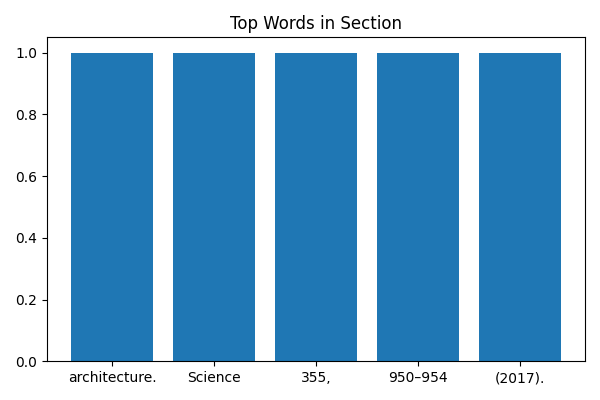
\includegraphics[width=0.8\textwidth]{D:\projects\mp 2 rag\autonomous rag\outputs\visual_45289be7e55a45e783f26d6c48264c68.png}
\end{figure}
\section{PCR}
Here's a simple summary of the section:

This section is about a way to store data in DNA using a device called the MinION. Here's how it works:

1. Take a file you want to store and make many copies of it using a process called PCR.
2. Mix the copies together and add special tags to the ends.
3. Sequence the mixed DNA using the MinION, which generates many reads (pieces of data).
4. Because the MinION makes more mistakes than other sequencing methods, you need to use many reads to get the correct data back.

The graph shows that the MinION makes more errors than other methods, but using more reads can help fix those errors and get the original data back.

Further reading: https://www.semanticscholar.org/search?q=PCR
\begin{figure}[h]
\centering
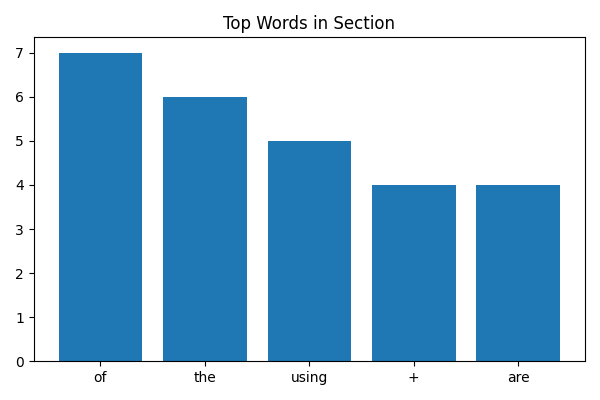
\includegraphics[width=0.8\textwidth]{D:\projects\mp 2 rag\autonomous rag\outputs\visual_f0c75e875f2841589e1e0e283048ce86.png}
\end{figure}
\section{8.	 Yazdi, S.M.H.T., Yuan, Y., Ma, J., Zhao, H. & Milenkovic, O. A rewritable, random-}
Here is a summary of the section in clear, simple terms:

This is a reference to a scientific study published in 2015 in a journal called Scientific Reports. The study is about a system that uses DNA to store data.

Further reading: https://www.semanticscholar.org/search?q=8.	%20Yazdi,%20S.M.H.T.,%20Yuan,%20Y.,%20Ma,%20J.,%20Zhao,%20H.%20&%20Milenkovic,%20O.%20A%20rewritable,%20random-
\begin{figure}[h]
\centering
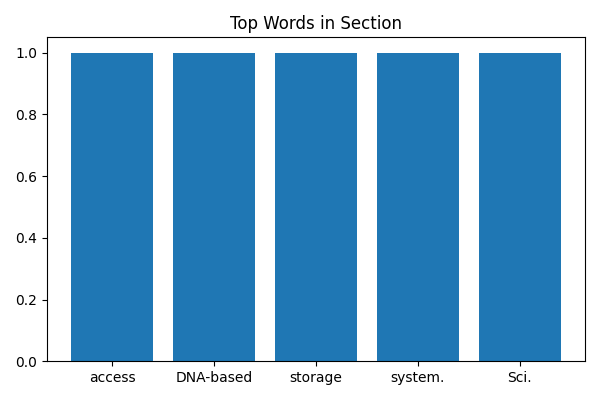
\includegraphics[width=0.8\textwidth]{D:\projects\mp 2 rag\autonomous rag\outputs\visual_efe4b4ffe7c240ee9bc021ff5ea98dab.png}
\end{figure}
\section{10.	Yazdi, S.M.H.T., Gabrys, R. & Milenkovic, O. Portable and error-free DNA-based}
This section appears to be a reference to a scientific paper. Here's a simple summary:

The reference is to a scientific article published in 2017 in a journal called "Scientific Reports". The article is about data storage and has the identifier "5011" in volume 7 of the journal.

Further reading: https://www.semanticscholar.org/search?q=10.	Yazdi,%20S.M.H.T.,%20Gabrys,%20R.%20&%20Milenkovic,%20O.%20Portable%20and%20error-free%20DNA-based
\begin{figure}[h]
\centering
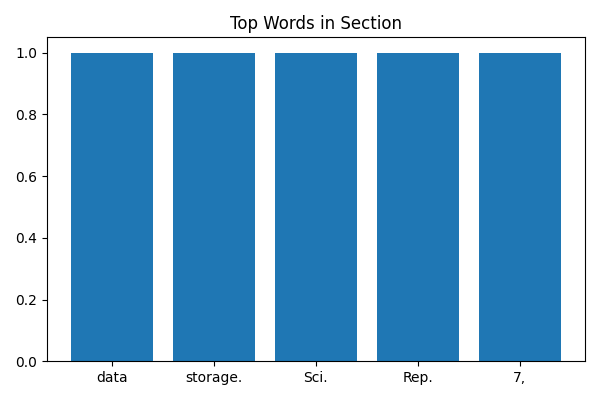
\includegraphics[width=0.8\textwidth]{D:\projects\mp 2 rag\autonomous rag\outputs\visual_abf2e34641ac48ff848d58046784cc2d.png}
\end{figure}
\section{11.	Kosuri, S. & Church, G.M. Large-scale de novo DNA synthesis: technologies and}
This is a reference to a scientific article. Here's a simple summary:

The article is about a scientific method or technique and its various uses. It was published in a journal called "Nature Methods" in 2014, in the 11th volume, on pages 499-507.

Further reading: https://www.semanticscholar.org/search?q=11.	Kosuri,%20S.%20&%20Church,%20G.M.%20Large-scale%20de%20novo%20DNA%20synthesis:%20technologies%20and
\begin{figure}[h]
\centering
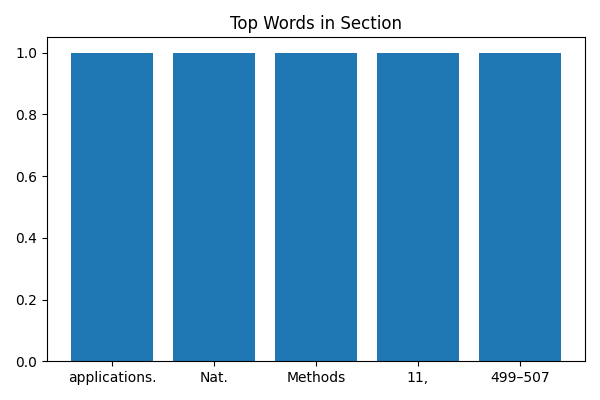
\includegraphics[width=0.8\textwidth]{D:\projects\mp 2 rag\autonomous rag\outputs\visual_5e37ca0f92084a6181928a539b2b3282.png}
\end{figure}
\section{12.	Xu, Q., Schlabach, M.R., Hannon, G.J. & Elledge, S.J. Design of 240,000 orthogonal}
Here is a summary of the section in clear, simple terms:

This is a reference to a scientific study published in 2009 in the journal Proceedings of the National Academy of Sciences of the United States of America (PNAS). The study is about using short pieces of DNA (called "25mer DNA barcode probes") to identify specific genes or organisms.

Further reading: https://scholar.google.com/scholar?q=12.	Xu,+Q.,+Schlabach,+M.R.,+Hannon,+G.J.+&+Elledge,+S.J.+Design+of+240,000+orthogonal
\begin{figure}[h]
\centering
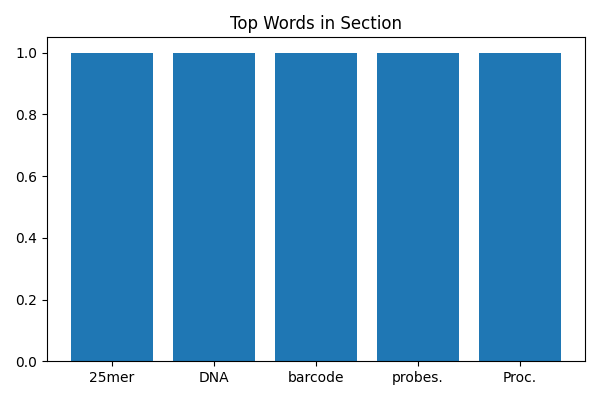
\includegraphics[width=0.8\textwidth]{D:\projects\mp 2 rag\autonomous rag\outputs\visual_fb32618fb89345289864d84c1a95ff85.png}
\end{figure}
\section{13.	Batu, T., Kannan, S., Khanna, S. & McGregor, A. Reconstructing strings from random}
Here is a summary of the section in clear, simple terms:

This is a reference to a research paper that was presented at a conference called SODA (Symposium on Discrete Algorithms) in 2004. The paper is titled "Traces" and it was published in the proceedings of the conference, which is a collection of papers presented at the event.

Further reading: https://arxiv.org/search/?query=13.	Batu,+T.,+Kannan,+S.,+Khanna,+S.+&+McGregor,+A.+Reconstructing+strings+from+random&searchtype=all
\begin{figure}[h]
\centering
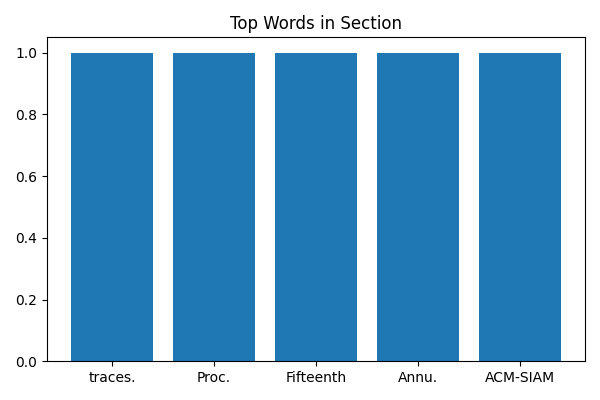
\includegraphics[width=0.8\textwidth]{D:\projects\mp 2 rag\autonomous rag\outputs\visual_9940174ae77447b280978171549b7369.png}
\end{figure}
\section{14.	Pellicer, J., Fay, M.F. & Leitch, I.J. The largest eukaryotic genome of them all? Bot.}
This section appears to be a citation or reference to a scientific article. Here's a simple summary:

This is a reference to a scientific paper that was published in two different places:

* In 2010, it was published in the "Journal of the Linnean Society" (volume 164, pages 10-15).
* The same paper is also being referenced in a 2018 issue of "Nature Biotechnology", with a specific identifier (doi:10.1038/nbt.4079).

Further reading: https://scholar.google.com/scholar?q=14.	Pellicer,+J.,+Fay,+M.F.+&+Leitch,+I.J.+The+largest+eukaryotic+genome+of+them+all?+Bot.
\begin{figure}[h]
\centering
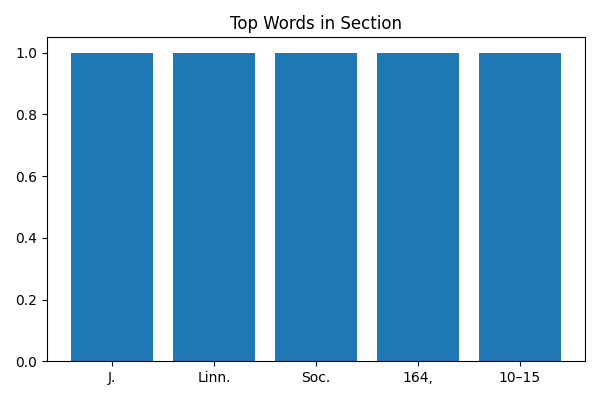
\includegraphics[width=0.8\textwidth]{D:\projects\mp 2 rag\autonomous rag\outputs\visual_a6a8de1fbc4545c59f9a67d8786c669e.png}
\end{figure}
\section{ONLINE METHODS}
Here's a simplified summary of the section:

**Amplifying DNA**

The researchers received a pool of synthetic DNA and amplified each file individually using a special protocol. They mixed the DNA with primers and an enzyme, then vortexed the mixture and split it into three tubes. They then used a thermocycler to amplify the DNA, following a specific temperature protocol. The resulting DNA was purified and the amount of DNA was measured.

**Preparing DNA for Sequencing**

The amplified DNA was then prepared for sequencing by adding special adapters and cleaning up the sample. The sample was then mixed with other samples in proportion to their size, and prepared for sequencing using a special protocol.

**Sequencing with Illumina**

The prepared sample was loaded into an Illumina sequencer, which reads the DNA sequence.

**Sequencing with Oxford Nanopore Technologies**

The researchers also used a different sequencing technology called Oxford Nanopore Technologies. They amplified the DNA using a special protocol, then assembled the amplified DNA into a single piece. They then sequenced the DNA using the Oxford Nanopore Technologies sequencer.

**Data Availability**

The researchers made their data available online, including the DNA sequences and the code used to analyze the data.

Further reading: https://www.semanticscholar.org/search?q=ONLINE%20METHODS
\begin{figure}[h]
\centering
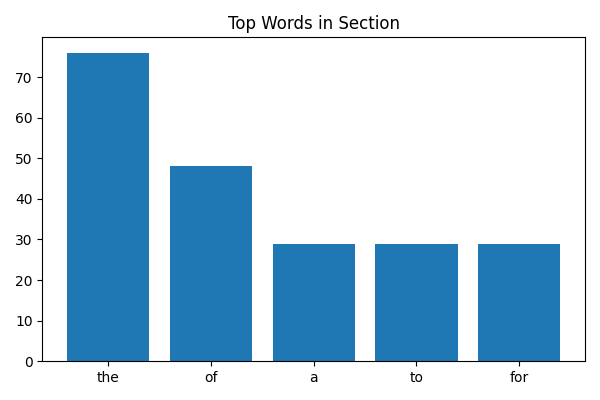
\includegraphics[width=0.8\textwidth]{D:\projects\mp 2 rag\autonomous rag\outputs\visual_afe8070352554653b4e20ce17cecf5dc.png}
\end{figure}
\section{15.	Zadeh, J.N. et al. NUPACK: analysis and design of nucleic acid systems. J. Comput.}
It appears that you've provided a citation for a scientific article. Here's a summary in simple terms:

This is a reference to a scientific paper published in a chemistry journal in 2011. The paper is on pages 170-173 of volume 32 of the journal.

Further reading: https://www.semanticscholar.org/search?q=15.	Zadeh,%20J.N.%20et%20al.%20NUPACK:%20analysis%20and%20design%20of%20nucleic%20acid%20systems.%20J.%20Comput.
\begin{figure}[h]
\centering
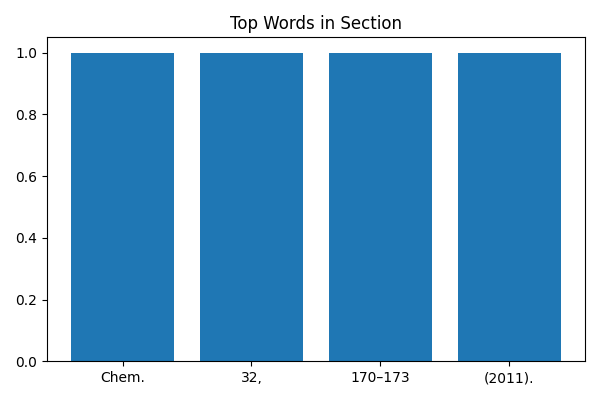
\includegraphics[width=0.8\textwidth]{D:\projects\mp 2 rag\autonomous rag\outputs\visual_c80197084dc04823a58302f2785d9901.png}
\end{figure}
\section{NATURE BIOTECHNOLOGY
E R R ATA}
Here is a summary of the section in clear, simple terms:

There was an error in an article published in Nature Biotechnology in 2018. The references at the end of the article were in the wrong order. The authors corrected the mistake by renumbering the references. They also removed one reference that was not needed. The corrections were made to the online and PDF versions of the article.

Further reading: https://www.semanticscholar.org/search?q=NATURE%20BIOTECHNOLOGY
E%20R%20R%20ATA
\begin{figure}[h]
\centering
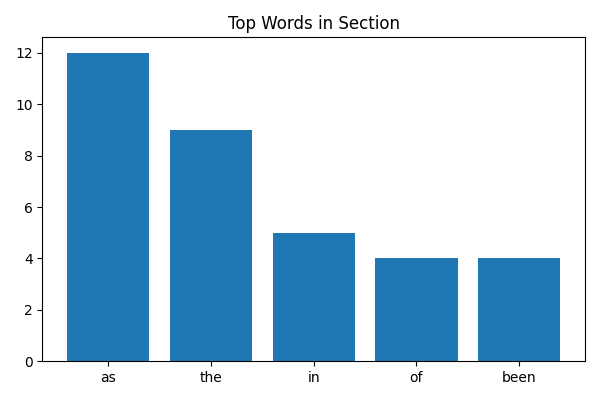
\includegraphics[width=0.8\textwidth]{D:\projects\mp 2 rag\autonomous rag\outputs\visual_48e04dc79243408da506626f94c68564.png}
\end{figure}
\end{document}